\documentclass[
11pt, % The default document font size, options: 10pt, 11pt, 12pt
%codirector, % Uncomment to add a codirector to the title page
]{charter} 


% El títulos de la memoria, se usa en la carátula y se puede usar el cualquier lugar del documento con el comando \ttitle
\titulo{Modelo de inteligencia artificial para la regulación de temperatura en equipos de inducción de hipotermia} 

% Nombre del posgrado, se usa en la carátula y se puede usar el cualquier lugar del documento con el comando \degreename
\posgrado{Carrera de Especialización en Inteligencia Artificial} 
%\posgrado{Carrera de Especialización en Internet de las Cosas} 
%\posgrado{Carrera de Especialización en Inteligencia Artificial}
%\posgrado{Maestría en Sistemas Embebidos} 
%\posgrado{Maestría en Internet de las cosas}
% IMPORTANTE: no omitir titulaciones ni tildación en los nombres, también se recomienda escribir los nombres completos (tal cual los tienen en su documento)
% Tu nombre, se puede usar el cualquier lugar del documento con el comando \authorname
\autor{Ing. Ezequiel Fernandez}

% El nombre del director y co-director, se puede usar el cualquier lugar del documento con el comando \supname y \cosupname y \pertesupname y \pertecosupname
\director{Título y Nombre del director}
\pertenenciaDirector{FIUBA} 

\codirector{} % para que aparezca en la portada se debe descomentar la opción codirector en los parámetros de documentclass
\pertenenciaCoDirector{}

% Nombre del cliente, quien va a aprobar los resultados del proyecto, se puede usar con el comando \clientename y \empclientename
\cliente{Marcelo Castiglione}
\empresaCliente{AmrrA Electromedicina}
 
\fechaINICIO{23 de abril de 2024}		%Fecha de inicio de la cursada de GdP \fechaInicioName
\fechaFINALPlan{11 de junio de 2024} 	%Fecha de final de cursada de GdP
\fechaFINALTrabajo{9 de diciembre de 2024}	%Fecha de defensa pública del trabajo final


\begin{document}

\maketitle
\thispagestyle{empty}
\pagebreak


\thispagestyle{empty}
{\setlength{\parskip}{0pt}
\tableofcontents{}
}
\pagebreak


\section*{Registros de cambios}
\label{sec:registro}


\begin{table}[ht]
\label{tab:registro}
\centering
\begin{tabularx}{\linewidth}{@{}|c|X|c|@{}}
\hline
\rowcolor[HTML]{C0C0C0} 
Revisión & \multicolumn{1}{c|}{\cellcolor[HTML]{C0C0C0}Detalles de los cambios realizados} & Fecha      \\ \hline
0      & Creación del documento    &\fechaInicioName \\ \hline
1      & Se completa hasta el punto 5 inclusive   & 7  de mayo de 2024 \\ \hline
2      & Se completa hasta el punto 9 inclusive  & 14  de mayo de 2024 \\ \hline
%		  Se puede agregar algo más \newline
%		  En distintas líneas \newline
%		  Así                                                    & {día} de {mes} de 202X \\ \hline
%3      & Se completa hasta el punto 12 inclusive                & {día} de {mes} de 202X \\ \hline
%4      & Se completa el plan	                                 & {día} de {mes} de 202X \\ \hline

% Si hay más correcciones pasada la versión 4 también se deben especificar acá

\end{tabularx}
\end{table}

\pagebreak



\section*{Acta de constitución del proyecto}
\label{sec:acta}

\begin{flushright}
Buenos Aires, \fechaInicioName
\end{flushright}

\vspace{2cm}

Por medio de la presente se acuerda con el \authorname\hspace{1px} que su Trabajo Final de la \degreename\hspace{1px} se titulará ``\ttitle'' y consistirá en la implementación de un modelo de inteligencia artificial prototipo para optimizar el rendimiento de un sistema de regulación de temperatura para uso en tratamientos de hipertermia e hipotermia. Además se analizará la incidencia de los distintos atributos en la predicción. El trabajo tendrá un presupuesto preliminar estimado de 600 horas y un costo estimado de \$ XXX, con fecha de inicio el \fechaInicioName\hspace{1px} y fecha de presentación pública el \fechaFinalName.

Se adjunta a esta acta la planificación inicial.

\vfill

% Esta parte se construye sola con la información que hayan cargado en el preámbulo del documento y no debe modificarla
\begin{table}[ht]
\centering
\begin{tabular}{ccc}
\begin{tabular}[c]{@{}c@{}}Dr. Ing. Ariel Lutenberg \\ Director posgrado FIUBA\end{tabular} & \hspace{2cm} & \begin{tabular}[c]{@{}c@{}}\clientename \\ \empclientename \end{tabular} \vspace{2.5cm} \\ 
\multicolumn{3}{c}{\begin{tabular}[c]{@{}c@{}} \supname \\ Director del Trabajo Final\end{tabular}} \vspace{2.5cm} \\
\end{tabular}
\end{table}




\section{1. Descripción técnica-conceptual del proyecto a realizar}
\label{sec:descripcion}

El objetivo de este proyecto será contar con un modelo de inteligencia artificial prototipo que estime la temperatura del agua que circula en un equipo utilizado para la inducción de hipotermia a pacientes neonatales. Además se hará foco en la incidencia de los parámetros que se disponen en el cálculo para aportar al conocimiento sobre estos tratamientos. Esto puede significar a futuro una mejora en un producto que desarrolla la empresa y brindar a quienes necesiten este tratamiento un desarrollo superador del mismo respecto a la actualidad. El proyecto será desarrollado dentro del marco del programa de vinculación. 

La empresa es AmrrA y los equipos en cuestión tienen el nombre Amrraterm HTF. Estos sistemas se utilizan con el propósito de inducir una hipotermia controlada en pacientes neonatales. Existen contextos en los cuales esto proporciona una mejor evolución de los pacientes. El principal caso de uso es el de pacientes que sufren hipoxia al nacer, esto es, falta de oxígeno en el cerebro. En estos casos, a temperatura corporal normal la interacción entre las neuronas es alta y se pueden desarrollar efectos adversos en la capacidad cerebral del paciente. Por esto un tratamiento estándar es el de inducir hipotermia por 72 horas a fin de minimizar los efectos que la hipoxia puede generar a futuro en los pacientes. 

Para lograr esto el procedimiento estándar es sedar al paciente y colocarlo dentro de una incubadora. Allí el mismo es envuelto en las mantas que forman parte del equipo. Por éstas circula agua destilada. El equipo regula la temperatura del agua en función de la temperatura objetivo, que suele ser de 33,5º C, y la actual del paciente. Una vez terminado el tratamiento de hipotermia, el equipo funciona en un modo llamado rampa, en el cual sube paulatinamente la temperatura hasta llegar a un estado normal.

Si bien existe un protocolo, que es el antes descrito, se dan ocasiones en las que se hace un mal uso del equipo, estableciendo como temperatura objetivo un valor inferior a los 33,5º C o utilizándolo en pacientes que no están correctamente sedados en incubadora. Estos casos podrían afectar los resultados del modelo por lo que deberían categorizarse.

En la actualidad la temperatura del agua es regulada por un algoritmo de lógica difusa. En un rango de pesos estándar (entre 2,5 kg y 3,5 kg) el algoritmo funciona correctamente, pero es posible que en pesos inferiores o superiores haya comportamientos que este proyecto pueda mejorar. Se desarrollará este modelo para evaluar si funciona mejor que el algoritmo actual en ese rango, en los valores inferiores o en los superiores de peso. 

Se utilizarán diversos datos para construir un modelo acorde al problema como el peso del paciente, la edad, la temperatura objetivo y las variaciones de temperatura del agua y paciente. Además de construir un modelo superador, también se busca detectar la incidencia de ciertos parámetros, como el peso del paciente, no utilizado por el algoritmo actual. Para evaluar el comportamiento del modelo se debe implementar un entorno, en algún lenguaje de programación a conveniencia de las partes, que permita evaluar y comparar resultados. 

En la figura \ref{fig:diagBloquesActual} se presenta un diagrama del funcionamiento del equipo actualmente. La temperatura del agua es regulada a través de un sistema térmico. Periódicamente un algoritmo de lógica difusa calcula la temperatura que debe tener el agua en el siguiente periodo.

\begin{figure}[htpb]
	\centering 
	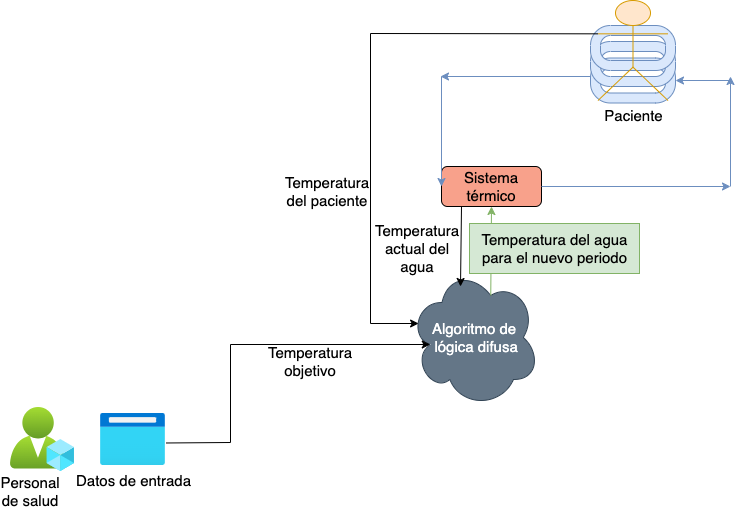
\includegraphics[width=.65\textwidth]{./Figuras/amrra-diagrama1.png}
	\caption{Diagrama en bloques del sistema actual.}
	\label{fig:diagBloquesActual}
\end{figure}

En la figura  \ref{fig:diagBloquesFuturo} se puede ver la incorporación de un modelo de inteligencia artificial en comparación con el actual.

\begin{figure}[htpb]
	\centering 
	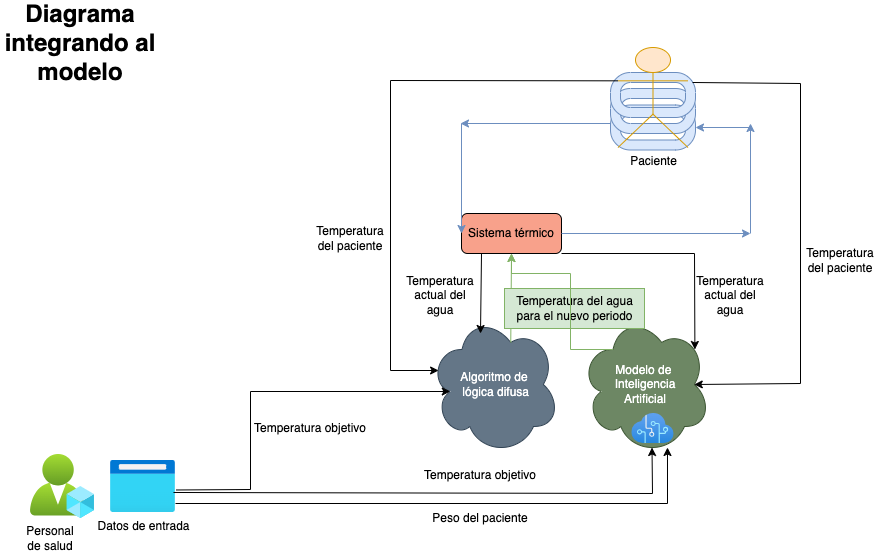
\includegraphics[width=.65\textwidth]{./Figuras/amrra-diagrama2.png}
	\caption{Diagrama en bloques del sistema integrando al modelo.}
	\label{fig:diagBloquesFuturo}
\end{figure}

Si bien existen artículos en la actualidad que analizan el uso de diversos modelos de \textit{machine learning} en contextos de hipotermia, la mayoría ponen el foco en estimar la mortalidad de los casos o en predecir potenciales casos de hipotermia. Estos enfoques son interesantes para evaluar los riesgos de someter al paciente bajo este tratamiento pero no son el objetivo de este proyecto. En este caso el foco estará en un modelo que regule de forma óptima la inducción a hipotermia de un paciente.

El presente proyecto se ve impulsado por buscar innovación utilizando tecnologías nuevas en un producto clave de la empresa. Se evaluará si esto resulta en una mejora en la calidad del producto y por esto en los tratamientos de los pacientes. Además se analizará la incidencia del peso y demás datos en el tratamiento para la correcta inducción de hipotermia, lo que aporta al conocimiento que se tiene actualmente sobre estos tratamientos. 

A futuro se llevará a cabo la integración del modelo resultante al sistema embebido del producto comercial Amrraterm HTF.

\section{2. Identificación y análisis de los interesados}
\label{sec:interesados}

\begin{table}[ht]
%\caption{Identificación de los interesados}
%\label{tab:interesados}
\begin{tabularx}{\linewidth}{@{}|l|X|X|l|@{}}
\hline
\rowcolor[HTML]{C0C0C0} 
Rol           & Nombre y Apellido & Organización 	& Puesto 	\\ \hline
Auspiciante   & Área de Ingeniería  &  AmrrA electromedicina &        Área de Ingeniería	\\ \hline
Cliente       &  Área de Ingeniería      & AmrrA electromedicina		&        Área de Ingeniería	\\ \hline
Impulsor      &  Marcelo  Castiglione &  AmrrA electromedicina	&        Área de Ingeniería	\\ \hline
Responsable   & \authorname       & FIUBA        	& Alumno 	\\ \hline
Colaboradores &  Ing. Laneri                 &      AmrrA electromedicina        	&   Área de Ingeniería	\\ \hline
Orientador    & \supname	      & \pertesupname 	& Director del Trabajo Final \\ \hline
Usuario final &   Médicos    &    Hospitales	&        -	\\ \hline
\end{tabularx}
\end{table}
 
\begin{itemize}
	\item Orientador: el director del trabajo es experto en la temática y va a ayudar con la exploración inicial y definición de estrategias para llegar a los objetivos.
	\item Impulsor: está muy interesado en el tema y en ayudar en lo que esté a su alcance.
	\item Usuario final: los médicos son quienes utilizarán los equipos y pueden  hacer comentarios acerca del uso de estos, pero también debemos mencionar a los pacientes que serán tratados.
\end{itemize}


\section{3. Propósito del proyecto}
\label{sec:proposito}
	
El propósito de este proyecto está orientado a cubrir los siguientes aspectos:
\begin{itemize}
	\item Desde un punto de vista funcional, consistirá de brindar un modelo de inteligencia artificial que estime cambio de temperatura óptimo para la salud del paciente en un instante.
	\item Desde un punto de vista conceptual, se desea analizar la incidencia del peso en este tratamiento.
	\item Desde un punto de vista personal, servirá como un medio formal para acreditar la Especialización en Inteligencia Artificial y como primer experiencia en un proyecto de esta temática en un ambiente cercano al laboral.	
\end{itemize}



\section{4. Alcance del proyecto}
\label{sec:alcance}

El alcance de este proyecto está orientado a desarrollar una solución de inteligencia artificial acorde al problema planteado. Se cubrirán los siguientes ejes de trabajo:

\begin{itemize}
	\item Entendimiento del problema y negocio: profundo aprendizaje sobre el contexto y rol que tendrá el modelo.
	\item Adquisición de datos y análisis de los mismos: análisis y preprocesamiento de los datos y generación de datos sintéticos en caso de escasez.
	\item Modelado: se evaluarán diversos modelos, buscando al de mejor rendimiento en función de poder predictivo y significado de los atributos.
	\item Resultado conceptual: se evaluará la incidencia de cada parámetro en las estimaciones del modelo.
	\item Visibilidad: se ofrecerá una forma de probar al modelo y de evaluarlo contra el algoritmo actual.
\end{itemize}

El presente proyecto no incluye: 
\begin{itemize}
	\item La incorporación del modelo a los equipos en funcionamiento.
	\item El despliegue del modelo en la nube.
	\item El desarrollo de una interfaz gráfica, una aplicación o una web.
\end{itemize}



\section{5. Supuestos del proyecto}
\label{sec:supuestos}

Para el desarrollo del presente proyecto se supone que: 

\begin{itemize}
	\item El desarrollo es alcanzable con los conocimientos actuales.
	\item El tiempo será suficiente para alcanzar los objetivos planteados. teniendo en cuenta imprevistos y cambios de enfoque posibles.
	\item Los accesos a la información y a los datos serán concedidos en tiempo y forma.
	\item La cantidad de datos disponibles y el pr procesamiento que pueda hacerse de los mismos será suficiente para un resultado aceptable.
\end{itemize}


\section{6. Requerimientos}
\label{sec:requerimientos}

\begin{enumerate}
	\item Requerimientos funcionales:
		\begin{enumerate}
			\item El modelo predecir el cambio de temperatura óptimo a aplicar.
			\item La salida del modelo debe ser conceptualmente análoga a la del algoritmo de lógica difusa utilizado actualmente a fin de poder compararlos.
			\item El modelo debe dar una respuesta en un tiempo promedio menor o igual a 10 veces el tiempo promedio de respuesta del algoritmo actual.
			\item El sistema debe permitir ingresar datos de forma manual y mostrar el resultado.
			\item Se debe calcular la incidencia del peso y de los demás atributos en la solución.
		\end{enumerate}
	\item Requerimientos conceptuales:
		\begin{enumerate}
			\item Deben utilizarse datos sintéticos en el entrenamiento.
		\end{enumerate}
	\item Requerimiento de testing:
		\begin{enumerate}
			\item Se deben ejecutar pruebas secuenciales con datos reales y mostrar una comparación entre los resultados del modelo a implementar y del algoritmo actual.
			\item Se deben comparar tiempos entre el modelo propuesto y el algoritmo actual.
			\item Se debe calcular una métrica a definir para calcular la performance del modelo.
		\end{enumerate}
	\item Requerimiento de documentación:
		\begin{enumerate}
			\item Se deben documentar las decisiones tomadas.
			\item Se deben documentar los resultados de las pruebas y las distintas métricas.
			\item Se requiere documentar el código y las formas de utilizar al sistema.
		\end{enumerate}
	\item Requerimiento asociados con regulaciones
		\begin{enumerate}
			\item Se requiere que los casos utilizados no expongan datos que infrinjan derechos de privacidad.
		\end{enumerate}
\end{enumerate}

\section{7. Historias de usuarios (\textit{Product backlog})}
\label{sec:backlog}

En esta sección se describirán algunas historias de usuarios ponderadas en un sistema de puntos, según el rol de cliente.

Para determinar los puntos de cada historia se definen los siguientes criterios:
\begin{itemize}
	\item Cantidad de trabajo:
	\begin{itemize}
		\item Baja: 1 punto.
		\item Media: 3 puntos.
		\item Alta: 5 puntos.
	\end{itemize}
	\item Complejidad del trabajo:
		\begin{itemize}
			\item Baja: 2 puntos.
			\item Media: 5 puntos.
			\item Alta: 13 puntos.
		\end{itemize}
	\item Incertidumbre del trabajo:
		\begin{itemize}
			\item Baja: 3 puntos.
			\item Media: 5 puntos.
			\item Alta: 10 puntos.
		\end{itemize}
\end{itemize}

La cantidad de puntos de una historia de usuario estará definida por el número en la sucesión de Fibonacci mas cercano y mayor o igual a la suma del puntaje de los tres criterios definidos.

\begin{itemize}
	\item Como cliente, quiero contar con un modelo que estime el cambio de temperatura en el equipo para tratamientos de hipotermia.
	\begin{itemize}
		\item Cantidad: de trabajo 5 puntos.
		\item Complejidad: 5 puntos.
		\item Incertidumbre: 10 puntos.
		\item Story Points: 5 + 5 + 10 = 20, tomando el siguiente de la sucesión de Fibonacci el puntaje es 21.
	\end{itemize}
	\item Como cliente, quiero conocer la incidencia del peso en el calculo de la variación de temperatura óptima para los pacientes.
		\begin{itemize}
			\item Cantidad: de trabajo 1 punto.
			\item Complejidad: 5 puntos.
			\item Incertidumbre: 5 puntos.
			\item Story Points: 1 + 5 + 5 = 11, tomando el siguiente de la sucesión de Fibonacci el puntaje es 13.
		\end{itemize}
\end{itemize}

\section{8. Entregables principales del proyecto}
\label{sec:entregables}

Los entregables del proyecto son:

\begin{itemize}
	\item Manual de uso e integración del sistema.
	\item Código fuente.
	\item Diagrama de funcionamiento del sistema.
	\item Informe de pruebas.
	\item Memoria del trabajo final.
\end{itemize}

\section{9. Desglose del trabajo en tareas}
\label{sec:wbs}

\begin{enumerate}
\item Planificación general del proyecto (50 h).
	\begin{enumerate}
	\item Redacción de la descripción técnica y propósito (20 h).
	\item Definición del alcance, riesgos y requerimientos (10 h).
	\item Planificación del desarrollo (20 h).
	\end{enumerate}
\item Exploración y preprocesamiento de datos (110 h).
	\begin{enumerate}
	\item Análisis exploratorio de los datos (10 h).
	\item Generación de datos sintéticos (40 h).
	\item Preprocesamiento y categorización de datos (40 h).
	\item Etiquetado de datos según contextos de uso (20 h).
	\end{enumerate}
\item Desarrollo del modelo (230 h).
	\begin{enumerate}
	\item Definición del criterio de medición y comparación de modelos (16 h).
	\item Selección de modelos a utilizar (16 h).
	\item Implementación de los modelos (40 h).
	\item Experimentación con los modelos (40 h).
	\item Comparación de resultados y elección de modelo a utilizar (8 h).	
	\item Optimización del modelo elegido (40 h).
	\item Refinamiento del modelo y entendimiento del comportamiento del mismo (40 h).
	\item Cálculo de la incidencia de los parámetros en la predicción (30 h).
	\end{enumerate}
\item Desarrollo del entorno donde se prueba el modelo (68 h).
\begin{enumerate}
	\item Definición del lenguaje (8 h).
	\item Desarrollo del entorno (30 h).
	\item Integración del entorno con los algoritmos a probar (30 h).
\end{enumerate}
\item Evaluación y pruebas comparativas (72 h).
	\begin{enumerate}
	\item Pruebas comparativas con el algoritmo actual (24 h).
	\item Generación de gráficos y documentación de pruebas (16 h).
	\item Análisis de resultados (16 h).
	\item Comparación de tiempos de respuesta de los algoritmos (16 h).
	\end{enumerate}
\item Elaboración de la memoria (80 h).
	\begin{enumerate}
	\item Escritura de la memoria final (40 h).
	\item Elaboración de la presentación para la exposición final (20 h).
	\item Escritura de la documentación técnica del modelo y su uso para el cliente (20 h).
	\end{enumerate}
\end{enumerate}

Cantidad total de horas: 610 h.

\section{10. Diagrama de Activity On Node}
\label{sec:AoN}

\begin{consigna}{red}
Armar el AoN a partir del WBS definido en la etapa anterior.

Una herramienta simple para desarrollar los diagramas es el Draw.io (\url{https://app.diagrams.net/}).
\href{https://app.diagrams.net}{Draw.io}


\begin{figure}[htpb]
\centering 
\includegraphics[width=.8\textwidth]{./Figuras/AoN.png}
\caption{Diagrama de \textit{Activity on Node}.}
\label{fig:AoN}
\end{figure}

Indicar claramente en qué unidades están expresados los tiempos.
De ser necesario indicar los caminos semi críticos y analizar sus tiempos mediante un cuadro.
Es recomendable usar colores y un cuadro indicativo describiendo qué representa cada color.

\end{consigna}

\section{11. Diagrama de Gantt}
\label{sec:gantt}

\begin{consigna}{red}
Existen muchos programas y recursos \textit{online} para hacer diagramas de Gantt, entre los cuales destacamos:

\begin{itemize}
\item Planner
\item GanttProject
\item Trello + \textit{plugins}. En el siguiente link hay un tutorial oficial: \\ \url{https://blog.trello.com/es/diagrama-de-gantt-de-un-proyecto}
\item Creately, herramienta online colaborativa. \\\url{https://creately.com/diagram/example/ieb3p3ml/LaTeX}
\item Se puede hacer en latex con el paquete \textit{pgfgantt}\\ \url{http://ctan.dcc.uchile.cl/graphics/pgf/contrib/pgfgantt/pgfgantt.pdf}
\end{itemize}

Pegar acá una captura de pantalla del diagrama de Gantt, cuidando que la letra sea suficientemente grande como para ser legible. 
Si el diagrama queda demasiado ancho, se puede pegar primero la ``tabla'' del Gantt y luego pegar la parte del diagrama de barras del diagrama de Gantt.

Configurar el software para que en la parte de la tabla muestre los códigos del EDT (WBS).\\
Configurar el software para que al lado de cada barra muestre el nombre de cada tarea.\\
Revisar que la fecha de finalización coincida con lo indicado en el Acta Constitutiva.

En la figura \ref{fig:gantt}, se muestra un ejemplo de diagrama de gantt realizado con el paquete de \textit{pgfgantt}. 
En la plantilla pueden ver el código que lo genera y usarlo de base para construir el propio.

Las fechas pueden ser calculadas utilizando alguna de las herramientas antes citadas. Sin embargo, el siguiente ejemplo
fue elaborado utilizando 
\href{https://docs.google.com/spreadsheets/d/1fBz8NhSpc4tkkhz3KjJCbh1nR_ltDkfEcZi4tZXduqs}{esta hoja de cálculo}.

Es importante destacar que el ancho del diagrama estará dado por la longitud del texto utilizado para las tareas 
(Ejemplo: tarea 1, tarea 2, etcétera) y el valor \textit{x unit}. Para mejorar la apariencia del diagrama, es necesario
ajustar este valor y, quizás, acortar los nombres de las tareas.

\begin{figure}[htpb]
  \begin{center}
    \begin{ganttchart}[
      time slot unit=day,
      time slot format=isodate,
      x unit=0.038cm,
      y unit title=0.7cm,
      y unit chart=0.6cm,
      milestone/.append style={xscale=4}
      ]{2021-03-05}{2021-12-16}
      \gantttitlecalendar*{2021-03-05}{2021-12-16}{year} \\
      \gantttitlecalendar*{2021-03-05}{2021-12-16}{month} \\
      \ganttgroup{Duración Total}{2021-03-05}{2021-12-16} \\
      %%%%%%%%%%%%%%%%%Organización
      \ganttgroup{Organización}{2021-03-05}{2021-04-16} \\
      \ganttbar{Planificación del proyecto}{2021-03-05}{2021-04-15} \\
      %%%%%%%%%%%%%%%%%Ejecución
      \ganttgroup{Ejecución}{2021-04-16}{2021-10-21} \\
      \ganttbar{Tarea 1}{2021-04-16}{2021-04-29} \\
      \ganttbar{Tarea 2}{2021-04-30}{2021-05-13} \\
      \ganttbar{Tarea 3}{2021-05-14}{2021-05-27} \\
      \ganttbar{Tarea 4}{2021-05-28}{2021-07-12} \\
      \ganttbar{Tarea 5}{2021-07-13}{2021-08-09} \\
      \ganttbar{Tarea 6}{2021-08-10}{2021-09-23} \\
      \ganttbar{Tarea 7}{2021-09-24}{2021-09-30} \\
      \ganttbar{Tarea 8}{2021-10-01}{2021-10-14} \\
      \ganttbar{Tarea 9}{2021-10-15}{2021-10-21} \\
      % %%%%%%%%%%%%%%%%%Finalización
      \ganttgroup{Finalización}{2021-10-22}{2021-12-16} \\
      \ganttbar{Memoria v1}{2021-10-22}{2021-11-04} \\
      \ganttbar{Memoria v2}{2021-11-05}{2021-11-18} \\
      \ganttbar{Memoria final}{2021-11-19}{2021-12-02} \\
      % La fecha del siguiente milestone es la fecha en que terminamos la memoria
      \ganttmilestone{Enviar memoria al director}{2021-12-02} \\
      \ganttbar{Elaborar la presentación}{2021-12-03}{2021-12-16} \\
      \ganttmilestone{Ensayo de la presentación}{2021-12-16} \\
      %%%%%%%%%%%%%%%%%%%%%%%%%%%%%%%%%%%%%%%%%%%%%%%%%%%%%%%%%%%%%%%
    \end{ganttchart}
  \end{center}
  \caption{Diagrama de gantt de ejemplo}
  \label{fig:gantt}
\end{figure}


\begin{landscape}
\begin{figure}[htpb]
\centering 
\includegraphics[height=.85\textheight]{./Figuras/Gantt-2.png}
\caption{Ejemplo de diagrama de Gantt (apaisado).} %Modificar este título acorde.
\label{fig:diagGantt}
\end{figure}

\end{landscape}

\end{consigna}


\section{12. Presupuesto detallado del proyecto}
\label{sec:presupuesto}

\begin{consigna}{red}
Si el proyecto es complejo entonces separarlo en partes:
\begin{itemize}
	\item Un total global, indicando el subtotal acumulado por cada una de las áreas.
	\item El desglose detallado del subtotal de cada una de las áreas.
\end{itemize}

IMPORTANTE: No olvidarse de considerar los COSTOS INDIRECTOS.

Incluir la aclaración de si se emplea como moneda el peso argentino (ARS) o si se usa moneda extranjera (USD, EUR, etc). Si es en moneda extranjera se debe indicar la tasa de conversión respecto a la moneda local en una fecha dada.

\end{consigna}

\begin{table}[htpb]
\centering
\begin{tabularx}{\linewidth}{@{}|X|c|r|r|@{}}
\hline
\rowcolor[HTML]{C0C0C0} 
\multicolumn{4}{|c|}{\cellcolor[HTML]{C0C0C0}COSTOS DIRECTOS} \\ \hline
\rowcolor[HTML]{C0C0C0} 
Descripción &
  \multicolumn{1}{c|}{\cellcolor[HTML]{C0C0C0}Cantidad} &
  \multicolumn{1}{c|}{\cellcolor[HTML]{C0C0C0}Valor unitario} &
  \multicolumn{1}{c|}{\cellcolor[HTML]{C0C0C0}Valor total} \\ \hline
 &
  \multicolumn{1}{c|}{} &
  \multicolumn{1}{c|}{} &
  \multicolumn{1}{c|}{} \\ \hline
 &
  \multicolumn{1}{c|}{} &
  \multicolumn{1}{c|}{} &
  \multicolumn{1}{c|}{} \\ \hline
\multicolumn{1}{|l|}{} &
   &
   &
   \\ \hline
\multicolumn{1}{|l|}{} &
   &
   &
   \\ \hline
\multicolumn{3}{|c|}{SUBTOTAL} &
  \multicolumn{1}{c|}{} \\ \hline
\rowcolor[HTML]{C0C0C0} 
\multicolumn{4}{|c|}{\cellcolor[HTML]{C0C0C0}COSTOS INDIRECTOS} \\ \hline
\rowcolor[HTML]{C0C0C0} 
Descripción &
  \multicolumn{1}{c|}{\cellcolor[HTML]{C0C0C0}Cantidad} &
  \multicolumn{1}{c|}{\cellcolor[HTML]{C0C0C0}Valor unitario} &
  \multicolumn{1}{c|}{\cellcolor[HTML]{C0C0C0}Valor total} \\ \hline
\multicolumn{1}{|l|}{} &
   &
   &
   \\ \hline
\multicolumn{1}{|l|}{} &
   &
   &
   \\ \hline
\multicolumn{1}{|l|}{} &
   &
   &
   \\ \hline
\multicolumn{3}{|c|}{SUBTOTAL} &
  \multicolumn{1}{c|}{} \\ \hline
\rowcolor[HTML]{C0C0C0}
\multicolumn{3}{|c|}{TOTAL} &
   \\ \hline
\end{tabularx}%
\end{table}


\section{13. Gestión de riesgos}
\label{sec:riesgos}

\begin{consigna}{red}
a) Identificación de los riesgos (al menos cinco) y estimación de sus consecuencias:
 
Riesgo 1: detallar el riesgo (riesgo es algo que si ocurre altera los planes previstos de forma negativa)
\begin{itemize}
	\item Severidad (S): mientras más severo, más alto es el número (usar números del 1 al 10).\\
	Justificar el motivo por el cual se asigna determinado número de severidad (S).
	\item Probabilidad de ocurrencia (O): mientras más probable, más alto es el número (usar del 1 al 10).\\
	Justificar el motivo por el cual se asigna determinado número de (O). 
\end{itemize}   

Riesgo 2:
\begin{itemize}
	\item Severidad (S): X.\\
	Justificación...
	\item Ocurrencia (O): Y.\\
	Justificación...
\end{itemize}

Riesgo 3:
\begin{itemize}
	\item Severidad (S):  X.\\
	Justificación...
	\item Ocurrencia (O): Y.\\
	Justificación...
\end{itemize}


b) Tabla de gestión de riesgos:      (El RPN se calcula como RPN=SxO)

\begin{table}[htpb]
\centering
\begin{tabularx}{\linewidth}{@{}|X|c|c|c|c|c|c|@{}}
\hline
\rowcolor[HTML]{C0C0C0} 
Riesgo & S & O & RPN & S* & O* & RPN* \\ \hline
       &   &   &     &    &    &      \\ \hline
       &   &   &     &    &    &      \\ \hline
       &   &   &     &    &    &      \\ \hline
       &   &   &     &    &    &      \\ \hline
       &   &   &     &    &    &      \\ \hline
\end{tabularx}%
\end{table}

Criterio adoptado: 

Se tomarán medidas de mitigación en los riesgos cuyos números de RPN sean mayores a...

Nota: los valores marcados con (*) en la tabla corresponden luego de haber aplicado la mitigación.

c) Plan de mitigación de los riesgos que originalmente excedían el RPN máximo establecido:
 
Riesgo 1: plan de mitigación (si por el RPN fuera necesario elaborar un plan de mitigación).
  Nueva asignación de S y O, con su respectiva justificación:
  \begin{itemize}
	\item Severidad (S*): mientras más severo, más alto es el número (usar números del 1 al 10).
          Justificar el motivo por el cual se asigna determinado número de severidad (S).
	\item Probabilidad de ocurrencia (O*): mientras más probable, más alto es el número (usar del 1 al 10).
          Justificar el motivo por el cual se asigna determinado número de (O).
	\end{itemize}

Riesgo 2: plan de mitigación (si por el RPN fuera necesario elaborar un plan de mitigación).
 
Riesgo 3: plan de mitigación (si por el RPN fuera necesario elaborar un plan de mitigación).

\end{consigna}


\section{14. Gestión de la calidad}
\label{sec:calidad}

\begin{consigna}{red}
Elija al menos diez requerimientos que a su criterio sean los más importantes/críticos/que aportan más valor y para cada uno de ellos indique las acciones de verificación y validación que permitan asegurar su cumplimiento.

\begin{itemize} 
\item Req \#1: copiar acá el requerimiento con su correspondiente número.

\begin{itemize}
	\item Verificación para confirmar si se cumplió con lo requerido antes de mostrar el sistema al cliente. Detallar.
	\item Validación con el cliente para confirmar que está de acuerdo en que se cumplió con lo requerido. Detallar. 
\end{itemize}

\end{itemize}

Tener en cuenta que en este contexto se pueden mencionar simulaciones, cálculos, revisión de hojas de datos, consulta con expertos, mediciones, etc.  

Las acciones de verificación suelen considerar al entregable como ``caja blanca'', es decir se conoce en profundidad su funcionamiento interno.  

En cambio, las acciones de validación suelen considerar al entregable como ``caja negra'', es decir, que no se conocen los detalles de su funcionamiento interno.

\end{consigna}

\section{15. Procesos de cierre}    
\label{sec:cierre}

\begin{consigna}{red}
Establecer las pautas de trabajo para realizar una reunión final de evaluación del proyecto, tal que contemple las siguientes actividades:

\begin{itemize}
	\item Pautas de trabajo que se seguirán para analizar si se respetó el Plan de Proyecto original:\\
	 - Indicar quién se ocupará de hacer esto y cuál será el procedimiento a aplicar. 
	\item Identificación de las técnicas y procedimientos útiles e inútiles que se emplearon, los problemas que surgieron y cómo se solucionaron:\\
	 - Indicar quién se ocupará de hacer esto y cuál será el procedimiento para dejar registro.
	\item Indicar quién organizará el acto de agradecimiento a todos los interesados, y en especial al equipo de trabajo y colaboradores:\\
	  - Indicar esto y quién financiará los gastos correspondientes.
\end{itemize}

\end{consigna}

\end{document}